\documentclass{beamer}

\usepackage{beamerthemeDresden}
\usepackage[frenchb]{babel}
\usepackage[utf8]{inputenc}
\usecolortheme{beaver}

\usepackage{listings}
\usepackage{xcolor}
\lstdefinestyle{base}{
  basicstyle=\ttfamily\color{black} \footnotesize,
  moredelim=**[is][\color{blue}]{@}{@},
  moredelim=**[is][\color{red}]{&}{&}
}

\setbeamertemplate{navigation symbols}{
\insertframenumber/
\inserttotalframenumber
}

\usepackage{color}
\definecolor{vert}{rgb}{0,0.5,0}
\definecolor{violet}{rgb}{0.5,0,0.5}

\usepackage{tikz}
\usetikzlibrary{calc,positioning,matrix,arrows,shapes.geometric,shapes.symbols,shapes.misc,shapes,automata,petri,decorations.markings,shadows}
\usepackage{array}
\usepackage{subfig}

%----------TIKZ
\usetikzlibrary{calc,arrows,shapes,automata,petri,positioning,decorations.markings,shadows}

\tikzset{
    use/.style={
    circle,draw=black,fill=black,scale=0.5,text=white
    },
    mpi/.style={
    rectangle,draw=black,fill=black,scale=0.8,text=white
    },
    provide/.style={
    circle,draw=black,fill=white,scale=0.5
    },
    component/.style={
    rectangle,rounded corners=3pt,draw=black
    },
    dcomponent/.style={
    rectangle,rounded corners=3pt,dashed,draw=black
    },
    progm/.style={rectangle,dashed, draw=black, thin, text width=10em, text centered,rounded corners, minimum height=2em},
  line/.style={draw, thin, ->, shorten >=2pt},
  purp/.style={rectangle, draw=violet,fill=violet!20, text width=10em, text centered,thin,rounded corners,inner sep=3pt},
  purp2/.style={rectangle, draw=violet,fill=violet!20, text width=15em, text centered,thin,rounded corners,inner sep=3pt},
}
%-------------

\def\pprec{\mathrel{\scalebox{.9}[1]{$\prec$}\mkern-3mu%
  \scalebox{.4}[1]{$\prec$}\mkern-5.5mu\scalebox{.4}[1]{$\prec$}}}

\makeatletter
    \newenvironment{withoutheadline}{
        \setbeamertemplate{headline}[default]
        \def\beamer@entrycode{\vspace*{-\headheight}}
    }{}
\makeatother

%-------------------------------------------------------------------
\title[The Multi-Stencil Language]{The Multi-Stencil Language: orchestrating stencils with a mesh-agnostic DSL}
\author[Hélène Coullon (INRIA), Julien Bigot (CEA), Christian Perez (INRIA)]{\underline{Hélène Coullon}, Julien Bigot, Christian Perez}
\institute[INRIA]{INRIA team Avalon\\Maison de la simulation (CEA)}
\date{$5{th}$ JLESC Workshop - 28th June 2016, Lyon}
%-------------------------------------------------------------------

\begin{document}

%---------------

\begin{frame}
    \titlepage
\end{frame}

%-------------------------------------------------------------
% INTRODUCTION / MOTIVATION
%-------------------------------------------------------------
\section{Introduction}
%-------------------------------------------------------------
\begin{frame}
\frametitle{Domain Specific Languages} % HPC DSL
\begin{block}{+ Domain Specific Languages}
Separation of concerns between the domain and its efficient implementation
\begin{itemize}
\item Easy language for the end-user
\item Implicit optimizations
\item Implicit parallelization
\end{itemize}
\end{block}
But none or only a few DSLs used in production !
\end{frame}
%-------------------------------------------------------------
\begin{frame}
\frametitle{Domain Specific Languages} % HPC DSL
\begin{alertblock}{- Domain Specific Languages}
\begin{itemize}
\item Choose a domain and a language more or less specific
\item Difficult to combine DSLs (interoperability)
\begin{itemize}
\item Eexascale applications = many specific domains and interactions
\item semantic / compilation / back-end codes
\end{itemize}
\item Difficult to maintain
\end{itemize}
\end{alertblock}
\end{frame}
%-------------------------------------------------------------
\begin{frame}
\frametitle{How to improve it ?} % HPC DSL
\begin{itemize}
\item Choose the good abstraction level to
\begin{itemize}
\item stay efficient
\item be used in many domains (find common meta-domains)
\end{itemize}
\item Choose good programming models for
\begin{itemize}
\item the compiler programming
\item the back-end
\end{itemize}
\item Try to reuse existing DSLs (compilation process or back-end codes)
\end{itemize}
% \textit{Delite (Scala)\\
% Composition and Reuse with Compiled Domain-Specific Languages\\
% ECOOP'13}
\end{frame}
%-------------------------------------------------------------

%-------------------------------------------------------------
\section{Multi-Stencil Language : Yet another DSL for stencils !}
%-------------------------------------------------------------
\begin{frame}
\frametitle{Multi-Stencil application}
\begin{center}
\resizebox{\textwidth}{!}{%
\begin{tikzpicture}
\def \n {5}
\def \radius {3cm}
\def \margin {8} % margin in angles, depends on the radius

  \node[purp2,align=center] (edp) at ({360/\n * (2 - 1)}:\radius) {Partial Differential Equations\\\scriptsize $\frac{\partial u(x,y,t)}{\partial t} = \frac{\partial^2 u(x,y,t)}{\partial x^2} + \frac{\partial^2 u(x,y,t)}{\partial y^2}$};
  \node[progm,align=center,right of=edp,node distance=6cm] (cond) {\scriptsize + specific behavior for\\\scriptsize boundary conditions};
  \path[line,dashed] (edp) -- (cond);
  \node[purp,align=center] (maillage) at ({360/\n * (1 - 1)}:\radius) {Mesh\\Time iterations};
  \path[->] (maillage) edge[<-,thin,shorten <=2pt,shorten >=2pt, bend right=40]  node [fill=white,align=center] {\scriptsize Time and space\\\scriptsize discretization} (edp.east);
  \path[] (edp.west) edge[thin,shorten <=2pt,shorten >=2pt, bend right=90]  node [draw,circle,fill=white] (plus) {\scriptsize +} (maillage.west);
  \node[purp,align=center, below of=plus, node distance=3.5cm] (sche) {Explicit\\numerical schemes\\\textcolor{red}{stencils}};
  \node[progm, text width=11em,align=center,right of=sche,node distance=5.5cm] (expl) {\scriptsize Iterative neighboorhood approximation of the phenomena};
  \path[line,dashed] (sche) -- (expl);
  \path[line] (plus) -- node [fill=white,align=center] {\scriptsize Numerical methods\\\scriptsize Finite difference/volume/elment} (sche);
\end{tikzpicture}
}
\end{center}
\end{frame}
%----------------
\begin{frame}
\frametitle{Multi-Stencil Language : Yet another DSL for stencils !}
\begin{block}{Inputs}
follow a descriptive grammar to simply declare
\begin{itemize}
\item the sequential order of computations
\item what is read and written by each computation
\item with or without a neighborhood access (stencil)
\end{itemize}
\end{block}
\begin{block}{Outputs}
\begin{itemize}
\item parallel pattern of the multi-stencil application
\item hybrid parallelism included: data and task parallelism
\item choice of parallel languages (MPI, OpenMP, StarPU, SkelGIS, Global Arrays etc.)
\item end-users have to fill computation functions into this pattern
\end{itemize}
\end{block}
\end{frame}
%----------------
\begin{frame}
\frametitle{Multi-Stencil Language : Yet another DSL for stencils !}
\begin{itemize}
\item Choosen abstraction level
\begin{itemize}
\item mesh-agnostic description language
\begin{itemize}
\item should be usable for unstructured, Cartesian, curvilinear meshes
\end{itemize}
\item description concerns splited from implementation concerns
\begin{itemize}
\item usable with many different parallel libraries or languages back-ends
\end{itemize}
\end{itemize}
\item Choosen programming models for back-end
\begin{itemize}
\item Component programming model (maintainability, portability and composability)
\item Task scheduling model (portability and efficiency)
\end{itemize}
\item Reuse of existing languages and DSLs
\begin{itemize}
\item Use of a Distributed Data Structure DSL (MPI) : SkelGIS
\item MPI and OpenMP (4.x)
\end{itemize}
\end{itemize}
\end{frame}
%-------------------------------------------------------------
\section{Few results}
%----------------
\begin{frame}
\frametitle{Shallow-water equations}
\begin{center}
Cartesian mesh / finite volume method\\Strong scaling 10k x 10k mesh with 1k iterations\\TGCC Curie, Thin nodes
\resizebox{7cm}{!}{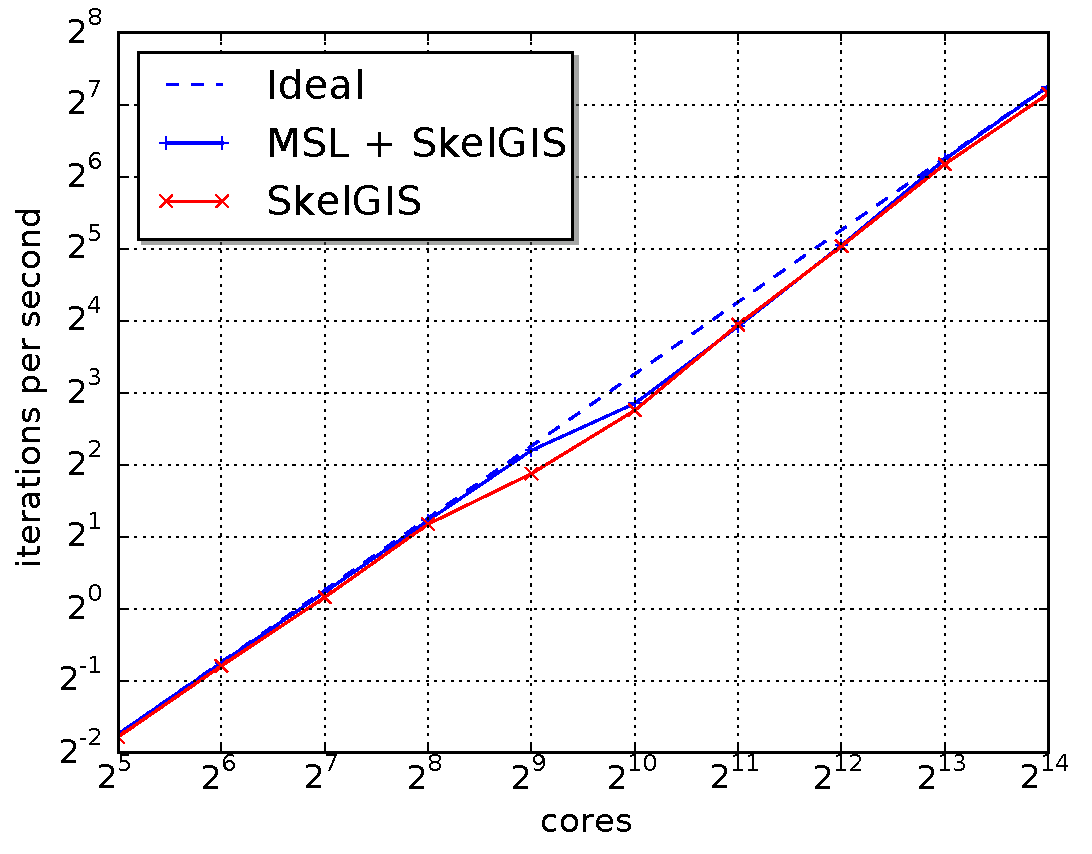
\includegraphics{./images/median_strong.pdf}}
\end{center}
\end{frame}
%----------------
\begin{frame}
\frametitle{Shallow-water equations}
\begin{center}
Cartesian mesh / finite volume method\\Weak scaling 400 x 400 per process\\TGCC Curie, Thin nodes
\resizebox{7cm}{!}{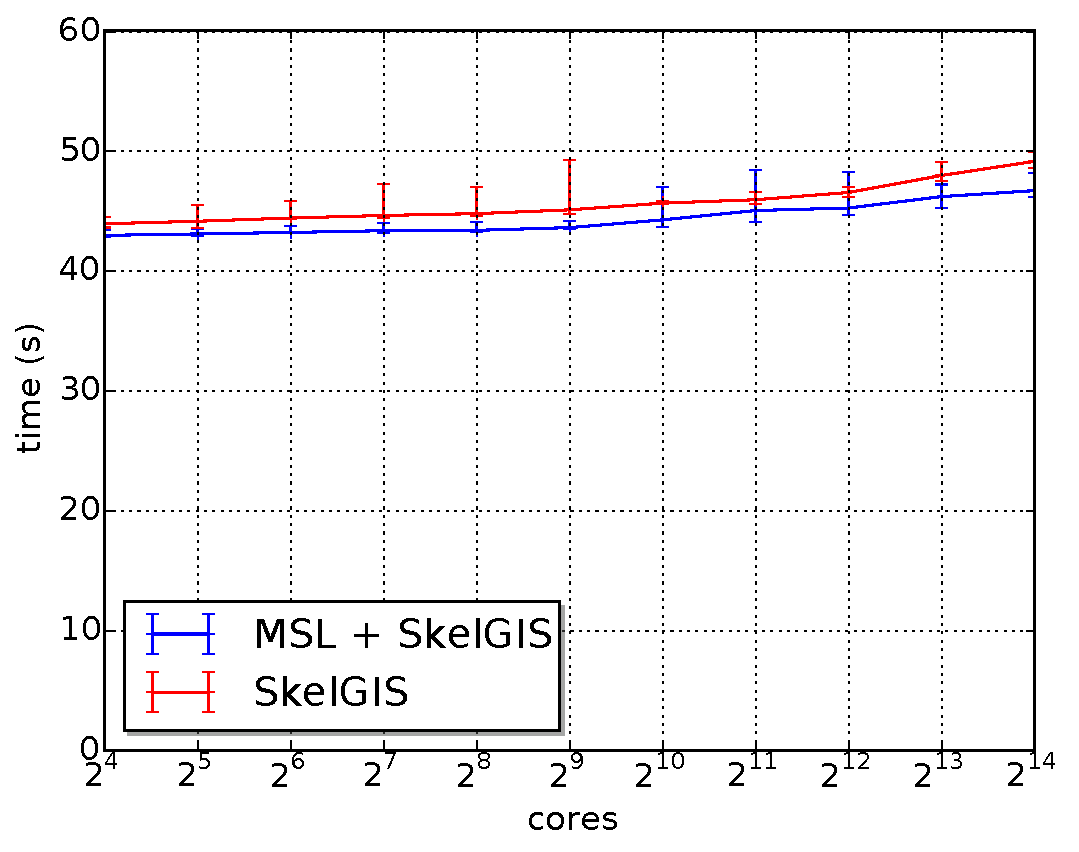
\includegraphics{./images/median_weak.pdf}}
\end{center}
\end{frame}
%----------------
% \begin{frame}
% \frametitle{Multi-Stencil Language : Yet another DSL for stencils !}
% \textbf{Improvment with data+task scheduling}
% \begin{center}
% \resizebox{8cm}{!}{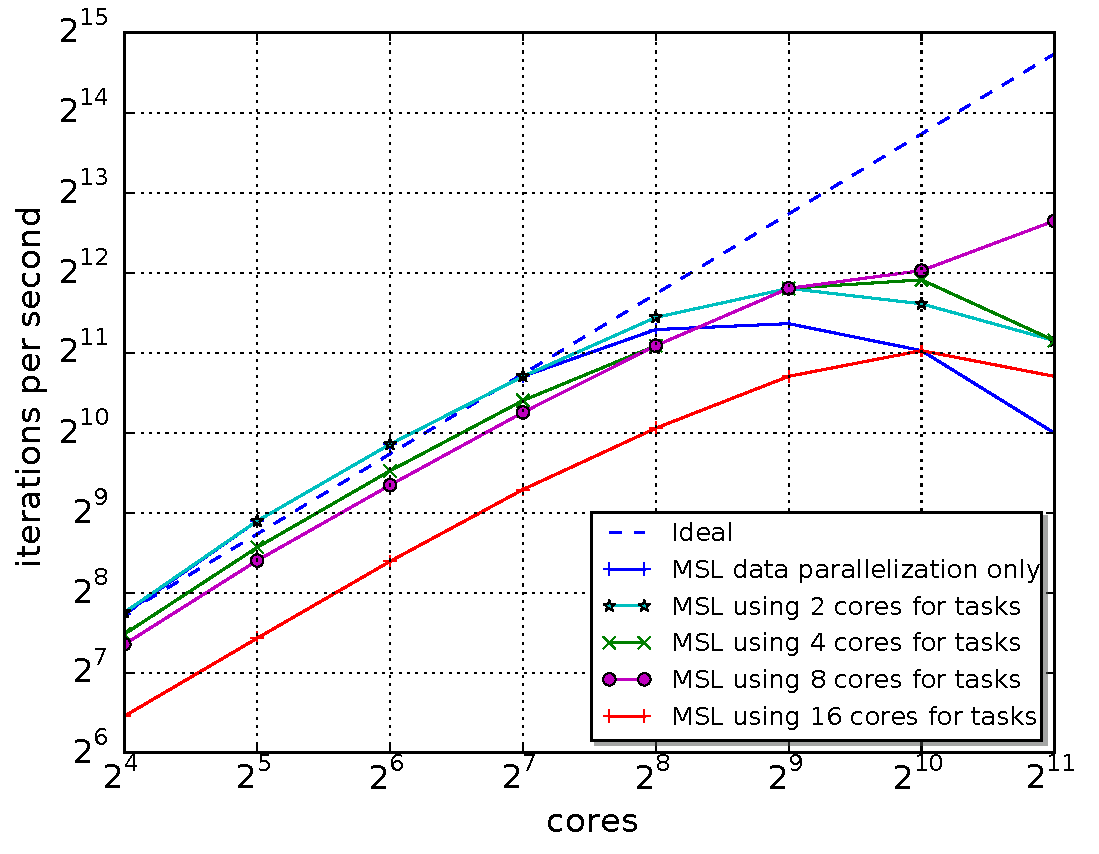
\includegraphics{./images/base_close_median.pdf}}
% \end{center}
% \end{frame}

%-------------------------------------------------------------
\begin{frame}
\frametitle{Work in progress and collaborations}
\begin{block}{Work in progress}
\begin{itemize}
\item different types of scheduling and back-end in MSL
\item combine MSL implementation choices to an energy-aware framework
\item new programming model back-end for MSL: combining component models and task models (Ph.D. Jérôme Richard)
\end{itemize}
\end{block}
\begin{block}{Collaborations}
\begin{itemize}
\item More application cases
\item Back-end programming model: component models and task scheduling (Components in OmpSs ?)
\item DSLs interoperability
\end{itemize}
\end{block}
\end{frame}
%-------------------------------------------------------------

% \begin{withoutheadline}
% \begin{frame}{}
% \begin{center}
% \huge Thank You !
% \end{center}
% \end{frame}
% \end{withoutheadline}

%----------------
\begin{frame}
\frametitle{MSL to Component-based runtime}
\begin{center}
\begin{tikzpicture}[remember picture]
  \node[rectangle,rounded corners=3pt,thick,inner sep=5pt,draw=black,dotted] (proc) {
    \begin{tikzpicture}[shorten >=1pt, node distance=2cm, on grid, auto]
     \node[component,solid] (D) at (0,0) {$Driver$};
     \node[provide,scale=0.5,solid] (Dp) at (-1,0) {};
     \node[solid] (Ds) at (-1.5,0) {start};
     \node[use,scale=0.5,solid,right=1.5cm of D] (Du1) {};
     \node[use,scale=0.5,solid,below=1.75cm of D] (Du2) {};
     \node[use,scale=0.5,solid,below=0.8cm of Du1] (Du3) {$m$};

     \node[provide,scale=0.5,solid,below=0.15 of Du2] (Tp) {};
     \node[component,solid,below=1.6cm of Tp] (T) {$Time$};
     \node[use,scale=0.5,solid,right=1cm of T] (Tu) {};

     \node[provide,scale=0.5,solid,right=0.15 of Tu] (Sp) {};
     \node[component,solid,right=1.5cm of Sp] (S) {$Scheduling$};
     \node[use,scale=0.5,solid,right=1.5cm of S] (Su) {};

     \node[provide,scale=0.5,solid,right=0.15 of Su] (Cp) {};
     \node[component,solid,double,right=2cm of Cp] (C) {$Kernel$};
     \node[use,scale=0.5,solid,above=0.8cm of C] (Cu) {};

     \node[provide,scale=0.5,solid,below right=0.2 of Du3] (Datap1) {};
     \node[provide,scale=0.5,solid,above=0.15 of Cu] (Datap2) {};
     \node[component,solid,double,above=0.8cm of Datap2] (Data) {$Data$};
     \node[use,scale=0.5,solid,above=0.8cm of Data] (Datau) {};

     \node[provide,scale=0.5,solid,right=0.15 of Du1] (DDSp1) {};
     \node[provide,scale=0.5,solid,above=0.15 of Datau] (DDSp2) {};
     \node[component,solid,above=0.8cm of DDSp2] (DDS) {$DDS$};
   
    \path[-]
      (Dp) edge [solid] node {} (D)
      (D) edge [solid] node {} (Du1)
          edge [solid] node {} (Du2)
          edge [solid] node {} (Du3)
      (DDSp1) edge [solid] node {} (DDS)
      (Tp) edge [solid] node {} (T)
      (T)  edge [solid] node {} (Tu)
      (Sp) edge [solid] node {} (S)
      (S) edge [solid] node {} (Su)
      (Datap2) edge [solid] node {} (Data)
      (Datap1) edge [solid] node {} (Data)
      (Data) edge [solid] node {} (Datau)
      (C) edge [solid] node {} (Cu)
      	  edge [solid] node {} (Cp)
      (DDSp2) edge [solid] node {} (DDS);
    \end{tikzpicture}
    };
    \node[mpi,scale=0.8,rounded corners=0pt,solid,right=0.5cm of proc] (mpidata) {};
    \node[solid,above=0.1cm of mpidata] (star2) {$*$};
    \node[solid,below=2.5cm of proc.west,anchor=west] (core) {\textit{\tiny{Duplicated on each processor/core}}};
    \path[-]
      (Data.east) edge node {} (mpidata);
  \end{tikzpicture}
\end{center}
\end{frame}

\end{document}

